\documentclass[10pt]{article}

\usepackage[
  paperwidth=5.5in,
  paperheight=8.5in,
  top=0.5in, bottom=0.5in, left=0.55in, right=0.55in,
  headsep=8pt, footskip=18pt
]{geometry}

\usepackage[T1]{fontenc}
\usepackage[utf8]{inputenc}
\renewcommand{\familydefault}{\sfdefault}
\usepackage{helvet}
\usepackage{graphicx}
\usepackage{xcolor}
\usepackage{tikz}
\usetikzlibrary{fadings}
\usepackage{fancyhdr}
\usepackage{titlesec}
\usepackage{enumitem}
\usepackage{microtype}
\usepackage{url}
\usepackage{hyperref}

\newcommand{\GameTitle}{RED SHIFT}
\newcommand{\GameByline}{CHARLES AVERILL}
\newcommand{\GameSite}{\href{https://charles.systems/}{CHARLES.SYSTEMS}}
\newcommand{\GameYear}{2026}

\definecolor{nesink}{HTML}{101018}
\definecolor{nesred}{HTML}{C82828}
\definecolor{nesblue}{HTML}{2038EC}
\definecolor{nesgray}{HTML}{7C7C7C}
\definecolor{nespaper}{HTML}{F4F1E8}
\pagecolor{nespaper}
\color{nesink}

\pagestyle{fancy}
\fancyhf{}
\renewcommand{\headrulewidth}{0.6pt}
\renewcommand{\footrulewidth}{0pt}
\fancyhead[L]{\footnotesize\bfseries\GameTitle}
\fancyhead[R]{\footnotesize\thepage}

\titleformat{\section}
  {\normalfont\Large\bfseries\color{nesred}}
  {}{0pt}{\MakeUppercase}
\titleformat{\subsection}
  {\normalfont\large\bfseries\color{nesblue}}
  {}{0pt}{\MakeUppercase}
\titlespacing*{\section}{0pt}{4pt}{6pt}
\setlist[itemize]{leftmargin=1.4em, itemsep=2pt, topsep=3pt}

\newcommand{\artbox}[3]{% width, height, label
  \begin{tikzpicture}
    \draw[dashed, nesgray, line width=0.5pt] (0,0) rectangle (#1,#2);
    \node[nesgray, font=\scriptsize] at (#1/2,#2/2) {#3};
  \end{tikzpicture}}

\linespread{1.08}
\setlength{\parindent}{0pt}
\setlength{\parskip}{4pt}

\begin{document}

\thispagestyle{empty}
\begin{center}
\vspace*{0.5in}

{\fontsize{48}{52}\selectfont\bfseries\color{nesred}\GameTitle}

\vspace{6pt}
{\large\bfseries\color{nesblue}INSTRUCTION BOOKLET}

\vspace{0.35in}
\begin{tikzpicture}
  \node[inner sep=0pt] {
    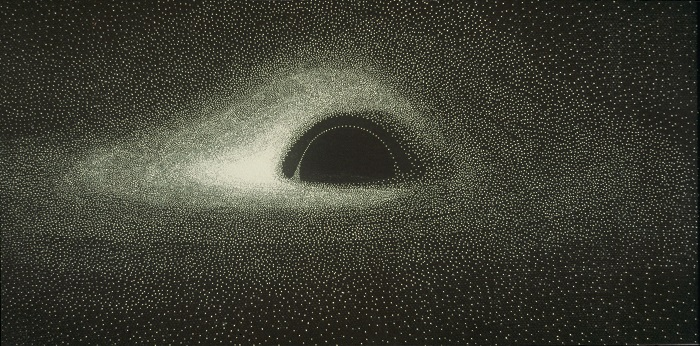
\includegraphics[width=3.4in]{images/cnrs.jpg}
  };
\end{tikzpicture}

\vfill

{\footnotesize \GameByline\ \textbullet\ \GameSite\ \textbullet\ \GameYear}
\end{center}
\clearpage

\section*{The Final Frontier}

Vie for survival on the endless drift of outer space!

In \GameTitle, you'll have to dodge, duck, dip, dive, and dodge oncoming asteroids and blast them to proceed.

As your score climbs, you will come face to face with scavengers and scoundrels alike, so be prepared for anything!

\vspace{6pt}
\section*{Contents}
\begin{itemize}[label={}]
  \item GETTING STARTED \dotfill 3
  \item YOUR SHIP \dotfill 3
  \item CONTROLS \dotfill 4
  \item HOW TO PLAY \dotfill 5
  \item PICKUPS \dotfill 6
  \item SCORING \dotfill 7
  \item HINTS \dotfill 7
\end{itemize}
\clearpage

\section*{Getting Started}

Make sure the power is OFF.

Insert the \GameTitle\ Game Pak and turn the power ON.

When the title screen appears, press START to begin.

After game over, press START to return to the title screen.

\vspace{6pt}
\section*{Your Ship}

\begin{center}
\includegraphics[width=2in,angle=35]{images/ship.png}\end{center}

Your RS-14X is a frenetic flyer, capable of reaching high speeds and drifting elegantly through dangerous asteroid fields.
Equipped with two sets of phased plasma rifles, it's sure to destroy anything in its path.

Your ship is equipped with four ENERGY SHIELDS that can handle one collision each.
Once all of your shields dissipate, you'll be on your own against the onslaught of asteroids!

\clearpage

\section*{Controls}

\begin{center}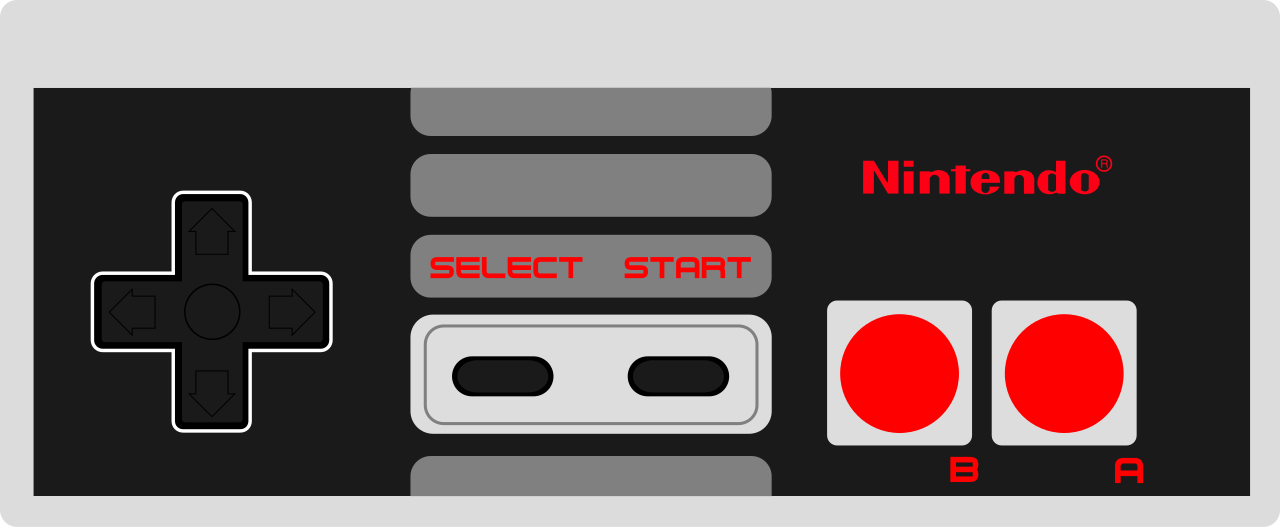
\includegraphics[width=0.6\textwidth]{images/nes_controller.png}\end{center}

\vspace{4pt}
\begin{tabular}{c l}
    \textbf{\textcolor{nesblue}{$\leftarrow$ / $\rightarrow$}} & Rotate the ship left or right \\
    \textbf{\textcolor{nesblue}{$\uparrow$}} & Fire thrusters to accelerate in the direction you are facing \\
    \textbf{\textcolor{nesblue}{$\downarrow$}} & Face retrograde \\
    \textbf{\textcolor{nesblue}{A}} & Fire blasters \\
    \textbf{\textcolor{nesblue}{START}} & Begin game or restart after game over \\
\end{tabular}

\vspace{3em}
\section*{How to Play}

Asteroids will drift into view from the edges of the screen.

Destroy many asteroids and collect the points and power-ups they drop to progress through the game.

\vfill
\textit{Handling hint:}
Hold $\downarrow$ to make the ship automatically turn to point against its own velocity.
Fire your thrusters once it aligns and you will decelerate.

\clearpage

\section*{Pickups}

Destroyed asteroids can drop these.
Fly over one to collect it.

\vspace{4pt}
\begin{tabular}{@{}p{0.9in}p{2.6in}@{}}
\centering 
\includegraphics[width=0.5in]{images/smallpoints.png} &
\vspace{-3em}\textbf{Small Points.}\newline Worth 4 base points. \\[10pt]

\centering 
\includegraphics[width=0.5in]{images/bigpoints.png} &
\vspace{-3.5em}\textbf{Large Points.}\newline Worth 8 base points. \\[10pt]

\centering 
\includegraphics[width=0.5in]{images/shield.png} &
\vspace{-3.5em}\textbf{Shield.}\newline Restores one shield level. Only appears when your shields are low. \\
\end{tabular}

\vspace{6pt}
\textit{Note:}
Pickups will disappear after a while.

\vspace{6pt}
\section*{Scoring}

Points build up on the counter at the top left of the screen.

When the count passes 999 it rolls over into the next order of magnitude.

\vspace{4pt}
\subsection*{The Multiplier}

Each pickup you collect increases your \emph{score multiplier}.

This multiplier augments the base points you acquire from pickups.

However, each time your ship is hit, your multiplier is lost.

Avoid projectiles and keep collecting pickups to increase your score even faster!

\clearpage

\thispagestyle{empty}
\vspace*{0.4in}
\begin{center}
{\Large\bfseries\color{nesred}\GameTitle}

\vspace{4pt}
{\footnotesize \GameByline}
\end{center}

\vfill

{\footnotesize
\textbf{COMPLIANCE.}
This product is an independent, non-commercial homebrew title.
It is not manufactured, sponsored, licensed, or endorsed by Nintendo.
``NES'' and ``Nintendo Entertainment System'' are trademarks of their respective owner, used here only descriptively.

\vspace{6pt}
\textbf{CARE.}
Keep the Game Pak clean and dry.
Do not store in direct sunlight or near sources of heat.
Do not clean with solvents.

\vspace{6pt}
\textbf{THANKS FOR PLAYING!}}

\vfill
\begin{center}
{\scriptsize \GameSite\ \textbullet\ PRINTED FOR HOMEBREW USE \textbullet\ \GameYear}
\end{center}
\clearpage

\end{document}
